%%%%%%%%%%%%%%%%%%%%%%%%%%%%%%%%%%%%%%%%%%%%%%%%%%%%%%%%
%%%%%%%%%%%%%%%%%%%%%%%%%%%%%%%%%%%%%%%%%%%%%%%%%%%%%%%%
\section[Pheno]{Feasibility study for a search of a \Tp~at LHC at 8 TeV}
\setcounter{tocdepth}{2}

\begin{frame}
\begin{center}
Feasibility study for a search of a \Tp~at LHC at 8 TeV
\end{center}
\end{frame}

\subsection{PHENO}

\begin{frame}{Motivation - Samples - Strategy}
\vspace{-.5cm}

\begin{columns}
\begin{column}{.50\textwidth}
\begin{block}{Motivation}
\begin{itemize}\tiny
\item Single produced \Tp~with mixings to light quark generations $\to$ Enhanced production cross section
\item Full hadronic channel:
  \begin{itemize}\tiny
  \item Difficult $\to$ huge backgrounds
  \item Highest number of expected events
  \item It is possible to reconstruct the \Tp~mass
  \item It needs techniques to choose the jets to reconstruct the \Tp
  \end{itemize}
\item $T'\to tH, tZ, bW$ and $Br(T'\to tH)=0.5$ $Br(H\to b\bar{b})=0.57$ $Br(t\to bq\bar{q}')=0.66$
\end{itemize}
\end{block}
\end{column}

\begin{column}{.50\textwidth}
%\begin{table}[htbH]
\begin{center}
\resizebox{\textwidth}{!}{
\begin{tabular}{||l|c|r||}
  \hline\hline
  Process & $\sigma_{\rm 8 TeV}$ (pb) & Expected Events \\ \hline
 Signal ($T'j$) & 0.2 & 700 \\
 \hline
  QCD (bbjjj) & 500 & 10,000,000 \\
  \W+jets & 37,509 & 750,180,000 \\
  \Z+jets & 3,503.71 & 70,074,200 \\
  \ttbar & 234 & 4,680,000 \\
  single-$t$ & 114.85 & 2,297,000 \\
  Di-boson & 96.82 & 1,936,400 \\
  \hline\hline
\end{tabular}
}
%\caption{Cross sections and expected number of events for background processes and signal for a luminosity of 20~$fb^{-1}$. \label{tab:xsec}}
\end{center}
%\end{table}
\vspace{-.5cm}
\begin{block}{}
\tiny $M(5j)$ $\to$ Five jets invariant mass as variable of interest
\end{block}
\end{column}
\end{columns}

\vspace{-.2cm}
\begin{block}{Strategy}
\begin{itemize}\tiny
\item Signal: 3 $b$-quarks and 2 light quarks $\to$ High b-jet multiplicity
\item Real Higgs boson and top quark in signal events
\item Method to have a good identification of the 5 jets coming from the \Tp:
\begin{itemize}\tiny
\item Tag b--jets and keep events with at least two.
\item b-jets pairs used to reconstruct the Higgs boson $\to$ ${\Delta R_{bb} <2.5}$ and pair with closest mass to the Higgs boson mass (125~\GeVcc)
\item b-jets removed from jets collection $\to$ jets pair with closest mass to the W-mass (80~\GeVcc) chosen to reconstruct the \W~boson 
\item Higgs and \W~boson jets removed from jet collection $\to$ the jet giving the closest mass to the top mass (172~\GeVcc), combined with W-jets, was used to reconstruct the top quark
\end{itemize}
\end{itemize}

\end{block}

\end{frame}

\begin{frame}{Selection}
\vspace{-.2cm}

\begin{columns}
\begin{column}{.50\textwidth}
\begin{block}{}
\begin{itemize}\scriptsize
\item \textit{Cut 0}: At least 6 jets with ${p_T > 30}$~GeV/c are required. At least five jets within $|\eta|<2.5$ and at least one jet within $2<|\eta|<5$. The \Tp~decays into five central jets. One associated jet in the forward direction. \\
\textbf{Figure}: $\eta$ distribution of the forward jet produced in association with \Tp. Signal sample is normalized to theoretical cross section and to 20~$fb^{-1}$.
\item \textit{Cut 1}: ${p_{T}(j_{1})>150}$~GeV/c, ${p_{T}(j_{2})>80}$~GeV/c, ${p_{T}(j_{3,4})>60}$~GeV/c
\item \textit{Cut 2}: $H_{T}>630$~GeV/c with $H_{T}=\sum |p_{T}(j)|$\\
\textbf{Figure}: Total hadronic energy for backgrounds (stacked) and signal (over--imposed) normalized to 20~$fb^{-1}$ luminosity. $H_{T}$ is higher in signal than in background events.
\end{itemize}
\end{block}
\end{column}

\begin{column}{.50\textwidth}
\begin{figure}[!Hhtbp]
  \begin{center}
    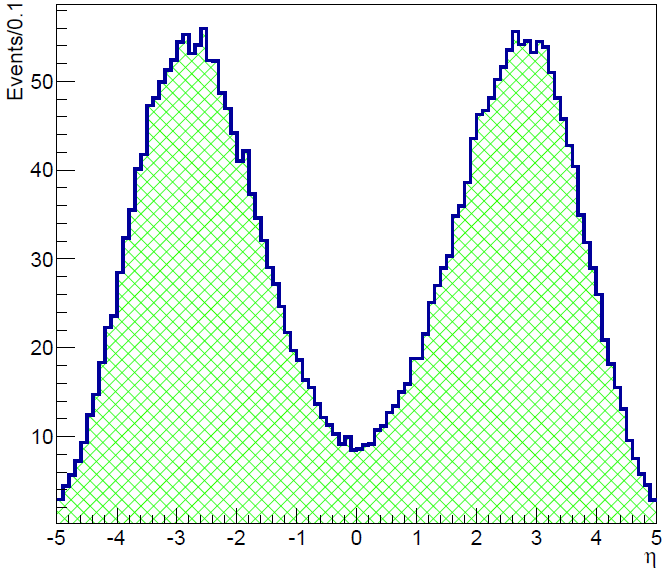
\includegraphics[width=0.75\textwidth]{../figs/Pheno/SixthJet.png}\\
    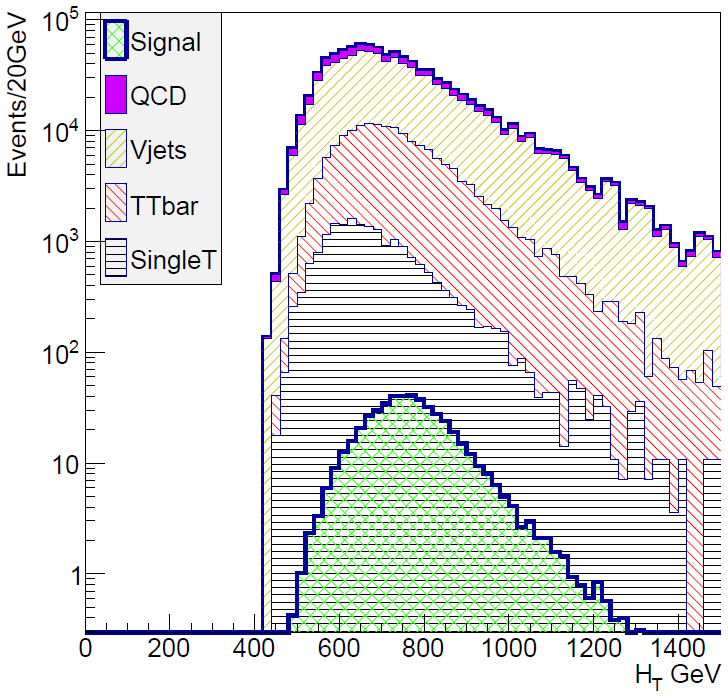
\includegraphics[width=0.75\textwidth]{../figs/Pheno/HT.png}
  \end{center}
\end{figure}
\end{column}
\end{columns}

\end{frame}

\begin{frame}{}
\vspace{-.2cm}

\begin{columns}
\begin{column}{.50\textwidth}
\begin{block}{}
\begin{itemize}\scriptsize
\item \textit{Cut 3}: At least two b-jets with effective CSV algorithm with medium working point.
\end{itemize}
\end{block}
\end{column}

\begin{column}{.50\textwidth}

\end{column}
\end{columns}

\end{frame}

\begin{frame}{}
\vspace{-.2cm}

\begin{columns}
\begin{column}{.50\textwidth}
\begin{block}{}
\begin{itemize}\scriptsize
\item 
\end{itemize}
\end{block}
\end{column}

\begin{column}{.50\textwidth}

\end{column}
\end{columns}

\end{frame}

\begin{frame}{}
\vspace{-.2cm}

\begin{columns}
\begin{column}{.50\textwidth}
\begin{block}{}
\begin{itemize}\scriptsize
\item 
\end{itemize}
\end{block}
\end{column}

\begin{column}{.50\textwidth}

\end{column}
\end{columns}

\end{frame}

\begin{frame}{}
\vspace{-.2cm}

\begin{columns}
\begin{column}{.50\textwidth}
\begin{block}{}
\begin{itemize}\scriptsize
\item 
\end{itemize}
\end{block}
\end{column}

\begin{column}{.50\textwidth}

\end{column}
\end{columns}

\end{frame}

\begin{frame}{}
\vspace{-.2cm}

\begin{columns}
\begin{column}{.50\textwidth}
\begin{block}{}
\begin{itemize}\scriptsize
\item 
\end{itemize}
\end{block}
\end{column}

\begin{column}{.50\textwidth}

\end{column}
\end{columns}

\end{frame}

\begin{frame}{}
\vspace{-.2cm}

\begin{columns}
\begin{column}{.50\textwidth}
\begin{block}{}
\begin{itemize}\scriptsize
\item 
\end{itemize}
\end{block}
\end{column}

\begin{column}{.50\textwidth}

\end{column}
\end{columns}

\end{frame}

\begin{frame}{}
\vspace{-.2cm}

\begin{columns}
\begin{column}{.50\textwidth}
\begin{block}{}
\begin{itemize}\scriptsize
\item 
\end{itemize}
\end{block}
\end{column}

\begin{column}{.50\textwidth}

\end{column}
\end{columns}

\end{frame}

\begin{frame}{}
\vspace{-.2cm}

\begin{columns}
\begin{column}{.50\textwidth}
\begin{block}{}
\begin{itemize}\scriptsize
\item 
\end{itemize}
\end{block}
\end{column}

\begin{column}{.50\textwidth}

\end{column}
\end{columns}

\end{frame}